\documentclass[UTF8]{ctexart}
\usepackage{cite}
\usepackage{graphicx}
\usepackage{subfigure}
\usepackage{booktabs}
\usepackage{geometry}
\usepackage{float}
\usepackage{amsmath}
\usepackage{lmodern}
\usepackage{multirow}
\geometry{a4paper,scale=0.75}
% \usepackage{cjk}
% \newcommand{\upcite}[1]{\textsuperscript{\textsuperscript{\cite{#1}}}}
\pagestyle{plain}
\begin{document}

\title{Straight network: A new network structure of landsat imagery cloud detection}
\author{王树立}
\date{\today}
\bibliographystyle{plain}
\maketitle
\section*{摘要}
云检测是应用遥感图像时重要的预处理步骤,一直是遥感领域中的研究热点。目前,很多方法基于单个像素的光谱,利用先验知识,通过设置合适的阈值,对像素进行分类。但这些方法往往没有考虑地物波段之间的关系,且无法利用图像的空间信息,很容易对一些高亮地物会造成误分,如冰雪。随着深度学习的发展,出现了一些利用神经网络做云识别的方法。但目前提出的神经网络大部分是为了处理灰色图或RGB图像的,这些方法没有考虑遥感图像多波段的特点,将现有的网络结构直接应用于遥感图像。且目前的神经网络算法在保持边缘细节与扩大感受野之间存在着难以协调的矛盾。本文中,我们提出了一种兼顾细节与感受野的新型网络结构,并充分考虑遥感图像多波段的优势,专门用于多波段的遥感图像云检测,但参数个数只有unet的二十分之一。我们用Landsat 8 Biome数据做训练并估计,取得了优于Fmask、并且与unet相当的实验结果。

\section[]{Introduction}
卫星遥感数据在当今社会的生产和生活中扮演者至关重要的角色,在农业产量估算\cite{prasad2006crop}、变化检测\cite{verbesselt2010detecting}、灾难评估\cite{joyce2009review}等方面发挥着重要的作用。随着科技的发展,遥感数据变得越来越多,且越来越容易获得。海量的多波段遥感数据也急切需要高效率和高鲁棒性的算法进行处理和数据挖掘。然而,在landsat数据集上,每年有高达40\%的像素被云覆盖\cite{ju2008availability},云层作为光学遥感图像的主要污染源,对遥感图像的应用造成了极大的限制。所以对云检测算法的研究一直是遥感领域中的热点。

云检测的任务是在遥感图像中逐像素地确定每一个像素点是否为云,若是简单地将像素分为云和非云两类,那么云检测就是一个输入一副图像,输出一个同等大小的二值化图像的过程。

光谱是地物最本质的特征之一,不同的地物有不同的辐射与反射特性,也会有很多的构造特征(如:NDVI,NDWI)。因此有很多基于单像素阈值的传统方法\cite{sun2018cloud}。Irish等人\cite{irish2006characterization}提出的ACCA使用 Landsat7 ETM +谱段 2- 6 的信息,获得暖云掩码,冷云掩码,非云掩码和雪掩码。算法所采用阈值的可靠性往往依赖于传感器精度和专家对所采集数据物理含义的理解。有静态阈值的,也有动态阈值的。此类方法实现简单,便于理解,可解释性强,在一般情况下可以取得较好的效果,但当地面覆盖了冰、雪、沙漠,或云为薄卷云、小积云时,云和地面难以区分。随着相关技术的发展,基于云纹理和空间特征的检测方法以及模式识别等技术在云检测方向上得到了广泛的应用。这类方法在具备先验知识的条件下可以获得较好的分类效果,但人为干预极大地影响检测效率。

基于同一地区时相相近的两幅或两幅以上影像进行云检测也是一类常见的方法。该类方法原理是认为,在高频率的观测下,相对于变化较快的云,陆地表面可以被看作是静态或缓变的背景。Zhe zhu 等\cite{zhu2014automated}提出的TMASK云掩膜算法首先根据FMASK识别出历史数据中清晰的像素,再选取三个波段,运用递归最小二乘方法,对选取出的三个波段利用正余弦函数进行拟合,最后计算当前值与预测值的差值判断每个像元是否为云。 
Goodwin等\cite{goodwin2013cloud}也利用时序数据构建了一种基于Landsat TM/ETM+的云检测算法,该算法综合利用影像的光谱、时相和上下文信息,在云检测方面精度比Fmask更高,但算法较为复杂,且需要大量无云的时间序列影像作为参考。
Ronggao Liu等\cite{liu2013generation}提出一种从MOD09时间序列产品中生成云掩膜的方法。利用蓝色波段和蓝色波段与短波红外波段之间的比值,对时间序列进行排序,以拐点值作为判别云与地物的门限。
基于时序的遥感图像云检测方法往往是非实时的,且需要依赖很多的其他数据。

近年来,深度学习在自然语言处理、降维、图像分类、目标检测、语义分割等方面取得了诸多成果。从AlexNet开始,深度学习开始席卷图像处理领域。一些文章将高分辨率图像切割成一张张小图或超像素,对图片或超像素进行分类,将其分为有云、无云两类或多云、少云、无云三类,但这降低了图像的分辨率。云检测其实是图像分割任务Pixel-level labeling tasks,图像分割可以定义为一种特定的图像处理技术,用于将图像划分为两个或两个以上有意义的区域。对于图像分割任务,输入一副图像,输出也是一副图像。

目前也有很多方法将全卷积网络应用于遥感图像的云检测\cite{chai2019cloud, jeppesen2019cloud},但很少有人会针对遥感图像多波段的特点对神经网络的结构进行针对性的设计。需要注意的是,这些神经网络模型是针对RGB图像设计的,而直接将为RGB图像设计的网络应用于多光谱遥感图像会有三个问题:1.因为RGB图像只有三个波段,针对RGB图像提出来的算法,空间信息无疑是神经网络提取的重点,这类网络往往通过加深层数以加大感受野,而对于识别大部分地物,尤其是检测云,过于考虑全局信息会对存储与计算造成巨大的浪费;2.感受野的增大往往意味着保持边缘细节能力的减弱,而对于云检测任务来说,我们在意的往往是这些边缘,一味地增加感受野可能会造成适得其反的效果;3.遥感图像有丰富的光谱信息,且光谱特征是地物最本质的特征,我们应该为光谱信息分配更多的计算资源。

在这篇文章中,我们基于U-Net,提出了一个新颖的、简单的、有效的网络,主要包括三部分。第一部分,考虑到复杂的下垫面是云检测中的难点,为了更好地处理复杂的下垫面,我们减少了encoder-decoder层数,注重局部空间特征。
第二部分,光谱特征提取部分,为了充分利用遥感图像多波段的特性,利用多层的1*1卷积核,对原始遥感图像进行波段特征提取,这样也可以保证边缘细节。
第三部分,引入注意力机制,将局部空间信息以attention的形式与像素光谱特征结合,得到最终的云掩膜图。
实验结果表明,该方法可以在模型参数大大减小的情况下,明显提高云检测精度。实验所用的所有代码均在github可见。

\section[]{Materials and Methods}
\subsection{Training and Evaluation Data}
我们采用的光学遥感卫星数据集来自NASA landsat8卫星。2013年2月11日,美国航空航天局(NASA) 成功发射Landsat-8卫星。Landsat-8卫星上携带两个传感器,分别是OLI陆地成像仪(Operational Land Imager)和TIRS热红外传感器(Thermal Infrared Sensor)。OLI提供9个波段,波段范围从0.43um到2.30um;TIRS提供地表温度数据,包括两个波段,波段范围从10.60um到12.51um,具体信息见表\ref{landsatBand}。landsat系列卫星每16天可以实现一次全球覆盖。
\begin{table}[H]
    \centering
    \begin{tabular}{c|c|c|c}
    \hline
    \hline
    传感器类型& 波段 &波长范围($\mu m$)& 空间分辨率\\
    \hline
    \multirow{9}*{OLI}& 1.Coastal& 0.433-0.453& 30\\
    ~&2.Blue& 0.450-0.515& 30\\
    ~&3.Green& 0.525-0.600& 30\\
    ~&4.Red& 0.630-0.680& 30\\
    ~&5.NIR& 0.845-0.885& 30\\
    ~&6.SWIR1& 1.56-1.66& 30\\
    ~&7.SWIR2& 2.1-2.3& 30\\
    ~&8.Pan& 0.5-0.68& 15\\
    ~&9.Cirrus& 1.36-1.39& 30\\
    \hline
    \multirow{2}*{OLI}& 10.TIRS1& 10.60-11.19& 100\\
    ~& 11.TIRS2& 11.50-12.51& 100\\
    \hline
    \hline
    \end{tabular}
    \caption{landsat8波段信息}
    \label{landsatBand}
    \end{table}


为了对模型进行训练与测试,我们利用已有的全球云和云影验证数据集
“L8 Biome Cloud Validation Masks”\cite{foga2017cloud_data},该数据集共有96景图片,包含8个种类的下垫面(including Barren, 
Forest,Grass/Crops, Shrubland, Snow/Ice, Urban, Water, Wetlands。

\begin{figure}[H]
    \centering
    \includegraphics[scale=0.5]{../pic/BiomeData.png}
    \caption{Global distribution of the 96 unique Landsat 8 Cloud Cover Assessment (CCA) scenes.}
    \label{fig:label}
\end{figure}

每景图片的标签均是人工标注,可信度较高。每个文件包含.TIF格式的Landsat 8 Level-1数据文件、质量文件和.img(ENVI)格式的真值标签,人工标志位如表\ref{BiomeFlag}所示。

\begin{table}[H]
    \centering
    \begin{tabular}{c|ccccc}
    \hline
    \hline
    value& 0& 64& 128& 192& 255\\
    \hline
    Interpretation&	Fill& Cloud Shadow& Clear &Thin Cloud& Cloud\\
    \hline
    \hline
    \end{tabular}
    \caption{L8 Biome 数据人工标注标志位}
    \label{BiomeFlag}
    \end{table}

根据云量百分比的多少,‘L8 Biome’中96景分为clear, midcloud, cloud三种,每种各占三分之一,云量低于35\%的为clear,云量高于65\%的为cloud,云量介于35\%与65\%之间的为midcloud。本文使用midcloud的所有数据,共32景做实验,每种地物有4景。数据我们将标签简单地分为云与非云两类,将每景L8图像均匀切割为256*256大小的小图,切割时过滤掉带填充值的图片,因此,图像边缘的填充像素并不会出现在训练与测试的步骤中。波段选择了除了全色波段的所有波段,共10个波段,训练集与测试集的比例为6:4,训练集有10247张子图,测试集有6932张子图。

\subsection{Background}

在提出我们的模型之前,我们先介近年来绍深度学习在语义分割方向的发展,了解模型的设计模式以及需要解决的问题。

Long提出FCN\cite{FCN}是CNN语义分割的开山之作,通过将普通CNN分类网络后的全连接层变为卷积层,实现了像素级别的分类。从此,不带全连接层的全卷积神经网络开始在语义分割任务上大放异彩。随后提出的U-Net\cite{ronneberger2015unet}是一种结构对称的网络,丰富了decoder部分。虽然在跳层连接这一部分,FCN用的是加操作(summation),U-Net用的是叠操作(concatenation),但encoder-decoder的框架是一致的。这两个算法的提出,奠定了encoder-decoder结构在语义分割领域的主流位置,其中,encoder的作用是提取空间特征,decoder的作用是解析空间特征,并将图像还原到原来的大小以获得像素级别的分类,跳层连接统筹兼顾感受野与空间分辨率。以后的网络,大部分都在这个框架下,如图\ref{fig:en-decoder}所示。

\begin{figure}[H]
    \centering
    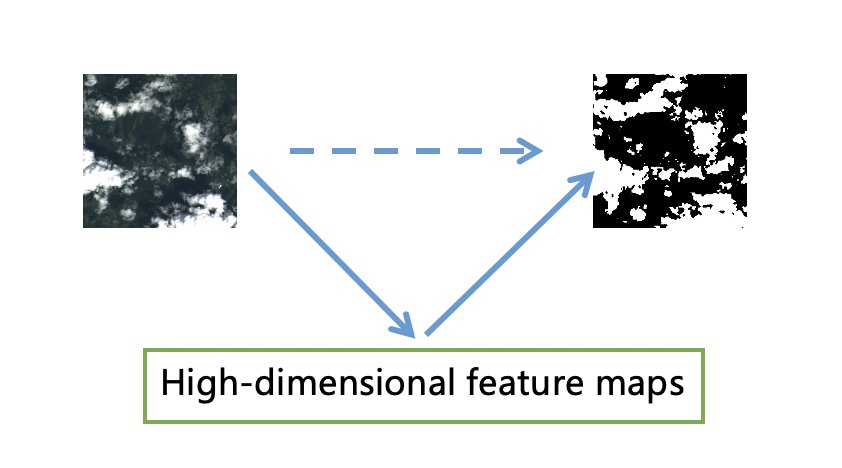
\includegraphics[scale=0.3]{../pic/en-decoder.jpg}
    \caption{encoder-decoder框架}
    \label{fig:en-decoder}
\end{figure}

需要注意的是,FCN与U-Net都用到了跳层连接,这其实揭示了端到端语义分割的一个主流矛盾:既需要全局的感受野来完成分类任务,又需要用局部信息和低层的低级视觉信息来达到准确的边缘分割。为了考虑更多的空间信息,需要获得更大的感受野,因此在重构过程中会产生粗糙的输出,最大池化层的存在则进一步降低了获得精细分割输出的机会。随着卷积神经网络深度的增加,特征图的空间分辨率降低,小目标的信息逐渐丢失。

为了解决这个矛盾,有很多方法对这个结构进行了改进。Shuai Zheng等人\cite{zheng2015conditional}提出了FCN-CRF,利用条件随机场对分割结果进行平滑与优化。Seg-Net\cite{badrinarayanan2015segnet}引入了一种新的上采样方式,叫做反池化,减少了大量参数,提升了计算性能,但准确率一般。Deeplab\cite{chen2014semantic, chen2017deeplab, chen2017rethinking}系列,用resnet作为基模型;利用空洞卷积在不损失分辨率和边缘信息的情况下增大感受野;引入一种类似于金字塔结构的模块--ASPP模块,以检测不同大小的物体。Zhou等人\cite{zhou2018unet++}提出的unet++,丰富了decoder结构,在每一层都加入了decoder,使用了浅层和深层的特征。也有将注意力机制应用于图像分割的方法\cite{zhang2018context, li2018pyramid, oktay2018attention},加权地学习全局信息,并保证局部信息。

\subsection{Network Architechture}

上一节提到,为了兼顾感受野与细节信息,这些基于灰度图与RGB图像设计的网络主要通过引入金字塔型的卷积核、注意力机制、丰富跳层连接、增加模型参数等方法。我们将神经网络应用于遥感图像,首先应该思考数据源的区别--多波段是遥感图像得天独厚的优势。为了完全挖掘遥感图像的信息,更好地利用landsat多波段的特点,我们调整了encoder-decoder结构,增加了直达通道,可以理解为一种特殊的跳层链接。
我们的模型结构如图\ref{fig_myModel},可以分为三部分:
\begin{figure}[H]
    \centering
    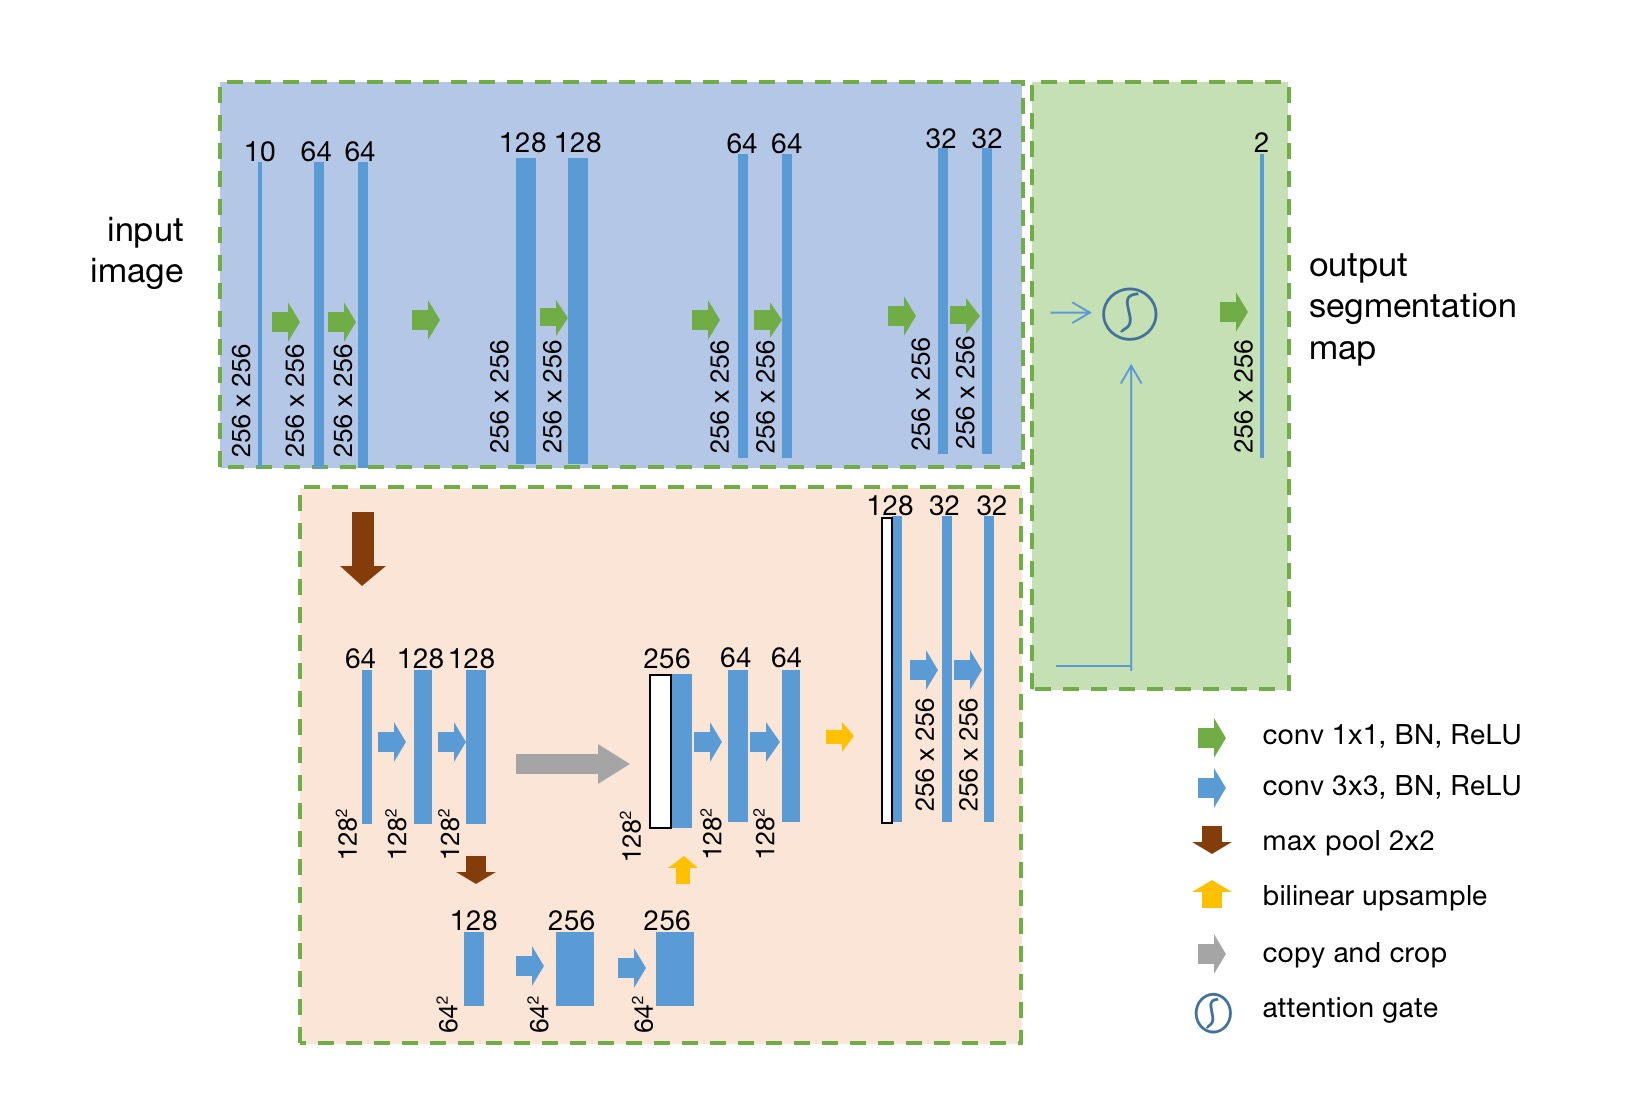
\includegraphics[scale=0.25]{../pic/model.jpg}
    \caption{our net architecture.}
    \label{fig_myModel}
\end{figure}

我们的模型整体上采用了encoder-decoder结构,与unet相比,主要有以下几方面改变:

1. 增加直达通道。直达通道里的所有卷积核的大小均为1*1,因此等价于一个多层的softmax网络。增加直达通道并不涉及空间信息的提取,专注于提取光谱信息,目的就是得到高分辨率的云掩膜图,以解决encoder-decoder结构天然的缺陷--在保持边缘细节与考虑全局信息之间存在着的以协调的矛盾。

\begin{figure}[H]
    \centering
    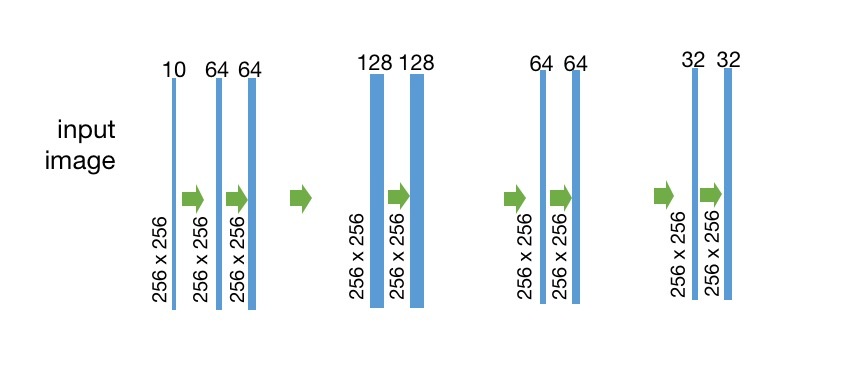
\includegraphics[scale=0.5]{../pic/straight.jpg}
    \caption[]{Straight access}
    \label{pic:straight}
\end{figure}

由于遥感图像特有的多波段特征,使得直达通道变得可能。若是不考虑图像的空间信息,对于遥感图像,我们使用决策树或者SVM也是可以对遥感图像的单个像素进行分类的,方法就是将每个像素单独地看作一个样本。事实上,很多方法就是这样做的,如zhu等人提出的FMask\cite{zhu2012object}。因此,我们的网络也具有良好的可替换性,通过将直达通道替换为传统的阈值法,可以将深度学习与传统经验完美地结合起来。

2. 减少了模型层数。unet为了提取全局信息,获得更大的感受野,设计了5层网络,共进行4次下采样,若不考虑3*3的卷积层,最深一层的每个像素包含了原始图片16*16像素大小的空间。我们认为遥感图像云检测应该更侧重局部信息,过深的层数不仅会造成资源的浪费,还会加剧边缘模糊的程度。所以我们将层数设计为3,意味着判断每个像素是否为云仅仅依靠其邻域4*4范围内的像素。

3. 加入局部注意力机制。近年来,有很多研究将attention机制加入到语义分割模型中来。在神经网络中,非线性主要来源于激活函数与池化,attention的引入增加了非线性,一部分人以此来解释attention的有效性。目前大多数网络会在感受野最大的卷积位置增加attention结构,以此来学习全局的有效信息。我们考虑到,在云检测任务中应该更加注重下垫面与局部信息,因此,我们只在decoder的最后一层加入了attention机制。

上采样的方式一般有四种:插值法,反卷积,反池化,超分辨率重建领域的亚像素卷积插值。双线性插值是目前在语义分割中用的比较多的一种插值方式,比如FCN中就是用的这种方法。在CNN上下文中,反卷积是卷积的逆过程,卷积用于提取空间信息,反卷积用于解析空间信息。在实现上,反卷积是卷积的转置,所以反卷积也叫做转置卷积。反池化是池化的逆过程,在池化过程中,记录下max-pooling在对应kernel中的坐标,在反池化过程中,将一个元素根据kernel进行放大,根据之前的坐标将元素填写进去,其他位置补0 。在下采样的时候记录max的位置,上采样的时候最大值的位置还原,其它位置填0。反池化是速度最快的上采样操作,计算量和参数也特别少,但是准确率一般。虽然理论上,由于反卷积具有更多的参数,所以反卷积可以更好的学习特征,但是有研究表明,如果参数配置不当,反卷积很容易出现输出feature map带有明显棋盘状的现象\cite{odena2016deconvolution},双线性差值可以取得与反卷积相同甚至更好的效果。因此,我们选择参数少且容易取得较好效果的双线性差值法。


本文中所有的激活函数都是ReLU函数。ReLU函数是一种分段线性函数,把所有的负值都变为0,而正值不变,这种操作被成为单侧抑制。单侧抑制使得神经网络中的神经元也具有了稀疏激活性。我们认为对于某种地物可以对某个特殊的指标有响应,而对其他指标就反应一般。所以ReLU实现稀疏后的模型能够更好地挖掘相关特征,且ReLU由于非负区间的梯度为常数,因此不存在梯度消失问题,使得模型的收敛速度维持在一个稳定状态。

\begin{equation}
    ReLU(x)=\left\{
    \begin{aligned}
        x, & &\text{if} & & x > 0 \\
        0, & &\text{if} & & x \leq 0
    \end{aligned}
    \right.
\end{equation}


\section[]{Experience and Result}

为客观评定算法的有效性和优越性,采用准确率,召回率,精确度,$F_1$值对结果进行评估。其中,准确率衡量像素分类正确的概率;召回率衡量属于云的像素中被分类正确的概率;精确度衡量被识别为云的像素中真正是云的概率;$F_1$值是召回率与精确度的调和平均数,常被用于二分类问题,可以有效衡量样本不均衡时检测结果的好坏。四个评价指标分别为:

\begin{equation}
    R_{accuracy} = \frac{TP + TN}{TP + TN + FP + FN}\label{acc}
\end{equation}
\begin{equation}
    R_{recall} = \frac{TP}{TP + FN}\label{recall}
\end{equation}
\begin{equation}
    R_{precision} = \frac{TP}{TP + FP}\label{precision}
\end{equation}
\begin{equation}
    R_{f1-score} = \frac{2 * R_{recall} * R_{precision}}{R_{recall} + R_{precision}}\label{f1}
\end{equation}
其中,TP为真正类(True Positive),即云被判为云;TN为真负类(True Negative),即非云被判为非云;FP为假正类(False Positive),即非云被判为云;FN为假负类(false Negative),云被判为非云。

本文将模型与landsat自带的QA波段、原始的UNet做比较。相比于QA波段,取得了8个百分点的性能提升;相比于原始的UNet,效果十分接近,但是我们的模型参数仅不到UNet的十分之一,更加轻量,具有更大的应用潜力。更详细的评估结果如表(\ref{tab_eval})所示。

\begin{table}[H]
    \centering
    \resizebox{\textwidth}{!}{
    \begin{tabular}{c|cccccccccc}
        \hline
        \hline
        model& evaluation& Barren& Forest& Grass/Crops& Shrubland& Snow/Ice& Urban& Water&  Wetlands& total\\
        \hline
        \multirow{4}*{our}
        &acc   &94.92 &94.55 &94.20 &95.17 &93.96 &94.85 &94.14 &94.40 &94.56\\
        &rec.  &94.19 &92.82 &88.84 &93.49 &90.77 &96.79 &90.29 &98.75 &93.81\\
        &prec. &97.47 &99.44 &94.73 &97.21 &94.51 &91.80 &94.56 &91.94 &95.39\\
        &F1    &95.80 &96.01 &91.69 &95.31 &92.60 &94.23 &92.37 &95.22 &94.60\\
        \hline
        \multirow{4}*{QA}
        &acc   &87.46 &95.20 &85.42 &90.34 &60.97 &83.05 &91.51 &90.78 &86.09\\
        &rec.  &90.85 &93.87 &68.03 &92.04 &92.21 &96.07 &92.22 &96.37 &91.45\\
        &prec. &88.99 &99.31 &88.85 &89.83 &51.74 &73.25 &86.97 &88.38 &82.89\\
        &F1    &89.91 &96.51 &77.05 &90.92 &66.29 &83.13 &89.52 &92.21 &86.96\\
        \hline
        \multirow{4}*{U-Net}
        &acc   &95.49 &95.73 &94.78 &95.91 &93.28 &94.56 &94.80 &94.30 &94.85\\
        &rec.  &96.35 &94.48 &89.25 &95.35 &87.97 &96.59 &93.88 &98.86 &94.09\\
        &prec. &96.32 &99.46 &95.97 &96.82 &95.52 &91.38 &92.94 &91.70 &95.01\\
        &F1    &96.33 &96.91 &92.49 &96.08 &91.59 &93.91 &93.41 &95.15 &94.48\\
        \hline
        \hline
    \end{tabular}}
    \caption{Evaluation results on the Biome dataset}
    \label{tab_eval}
\end{table}

在大部分情况下,我们的模型与U-Net相差无几。但仔细观察可以发现,我们的模型对于碎云、细节有良好的检测与保持能力。如图\ref{Fig.main}所示,(a)(b)(c)(d)分别为landsat真彩色图、人工标签、我们模型的云掩膜图、U-Net的云掩膜图,(e)(f)(g)(h)分别为放大之后的局部小图。我们的模型由于有直达通道的存在,对细节有较好的保持,对碎云有良好的识别;同时由于引入attention,也考虑到了图像的空间信息,能以极少的参数在整体上达到与U-Net相近的效果。

\begin{figure}[H]
    \centering  %图片全局居中

    \subfigure[RGB]{
    \label{Fig.sub.1}
    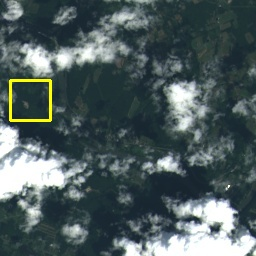
\includegraphics[width=0.2\textwidth]{../log/tmp_color.jpg}}
    \subfigure[mask]{
    \label{Fig.sub.2}
    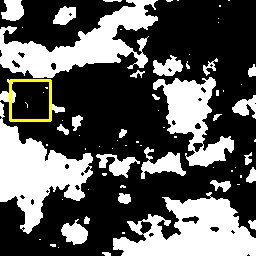
\includegraphics[width=0.2\textwidth]{../log/tmp_mask.jpg}}
    \subfigure[our]{
    \label{Fig.sub.3}
    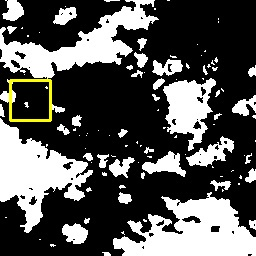
\includegraphics[width=0.2\textwidth]{../log/tmp_my.jpg}}
    \subfigure[U-Net]{
    \label{Fig.sub.4}
    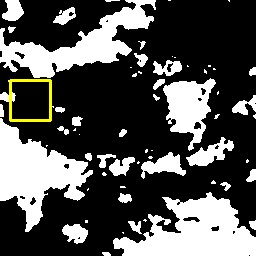
\includegraphics[width=0.2\textwidth]{../log/tmp_unet.jpg}}
    \subfigure[RGB]{
    \label{Fig.sub.5}
    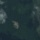
\includegraphics[width=0.2\textwidth]{../log/tmp_cut_color.jpg}}
    \subfigure[mask]{
    \label{Fig.sub.6}
    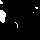
\includegraphics[width=0.2\textwidth]{../log/tmp_cut_mask.jpg}}
    \subfigure[our]{
    \label{Fig.sub.7}
    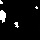
\includegraphics[width=0.2\textwidth]{../log/tmp_cut_my.jpg}}
    \subfigure[U-Net]{
    \label{Fig.sub.8}
    
\includegraphics[width=0.2\textwidth]{../log/tmp_cut_unet.jpg}}

    \caption{Main name}
    \label{Fig.main}
\end{figure}


\section[]{Conclusion}
云检测一直是遥感领域的研究热点与难点。本文提出了一种基于encoder-deconder结构改进的新的遥感图像云检测模型。该模型充分利用遥感图像多波段的特点,通过增加直达通道,并引入注意力机制,在保持边缘细节与扩大感受野之间寻找矛盾的解决方法,并在landsat8数据集上达到了94\%的准确率,基本还原了输入影像的细节信息。后续将继续优化直达通道与空间信息提取部分,并尝试深度学习与传统方法结合,以实现更加精确的遥感图像云检测。
\bibliography{./ref.bib}
\end{document}
